%%%%%%%%%%%%%%%%%%%%%%%%%%%%%%%%%%%%%%%%%
% Short Sectioned Assignment LaTeX Template Version 1.0 (5/5/12)
% This template has been downloaded from: http://www.LaTeXTemplates.com
% Original author:  Frits Wenneker (http://www.howtotex.com)
% License: CC BY-NC-SA 3.0 (http://creativecommons.org/licenses/by-nc-sa/3.0/)
%%%%%%%%%%%%%%%%%%%%%%%%%%%%%%%%%%%%%%%%%

%----------------------------------------------------------------------------------------
%	PACKAGES AND OTHER DOCUMENT CONFIGURATIONS
%----------------------------------------------------------------------------------------

\documentclass[paper=a4, fontsize=11pt]{scrartcl} % A4 paper and 11pt font size

% ---- Entrada y salida de texto -----

\usepackage[T1]{fontenc} % Use 8-bit encoding that has 256 glyphs
\usepackage[utf8]{inputenc}
%\usepackage{fourier} % Use the Adobe Utopia font for the document - comment this line to return to the LaTeX default

% ---- Idioma --------

\usepackage[spanish, es-tabla]{babel} % Selecciona el español para palabras introducidas automáticamente, p.ej. "septiembre" en la fecha y especifica que se use la palabra Tabla en vez de Cuadro

% ---- Otros paquetes ----

\usepackage{url} % ,href} %para incluir URLs e hipervínculos dentro del texto (aunque hay que instalar href)
\usepackage{amsmath,amsfonts,amsthm} % Math packages
%\usepackage{graphics,graphicx, floatrow} %para incluir imágenes y notas en las imágenes
\usepackage{graphics,graphicx, float} %para incluir imágenes y colocarlas

\usepackage{enumitem}

% Para hacer tablas comlejas
%\usepackage{multirow}
%\usepackage{threeparttable}

% Para utilizar pseudocódigo
\usepackage{algorithm}
\usepackage{algorithmic}
\usepackage{algorithmicx}
\usepackage{listings}

%\usepackage{sectsty} % Allows customizing section commands
%\allsectionsfont{\centering \normalfont\scshape} % Make all sections centered, the default font and small caps

\usepackage{fancyhdr} % Custom headers and footers
\pagestyle{fancyplain} % Makes all pages in the document conform to the custom headers and footers
\fancyhead{} % No page header - if you want one, create it in the same way as the footers below
\fancyfoot[L]{} % Empty left footer
\fancyfoot[C]{} % Empty center footer
\fancyfoot[R]{\thepage} % Page numbering for right footer
\renewcommand{\headrulewidth}{0pt} % Remove header underlines
\renewcommand{\footrulewidth}{0pt} % Remove footer underlines
\setlength{\headheight}{13.6pt} % Customize the height of the header

\numberwithin{equation}{section} % Number equations within sections (i.e. 1.1, 1.2, 2.1, 2.2 instead of 1, 2, 3, 4)
\numberwithin{figure}{section} % Number figures within sections (i.e. 1.1, 1.2, 2.1, 2.2 instead of 1, 2, 3, 4)
\numberwithin{table}{section} % Number tables within sections (i.e. 1.1, 1.2, 2.1, 2.2 instead of 1, 2, 3, 4)

\setlength\parindent{0pt} % Removes all indentation from paragraphs - comment this line for an assignment with lots of text

\newcommand{\horrule}[1]{\rule{\linewidth}{#1}} % Create horizontal rule command with 1 argument of height


%----------------------------------------------------------------------------------------
%	TÍTULO Y DATOS DEL ALUMNO
%----------------------------------------------------------------------------------------

\title{	
\normalfont \normalsize 
\textsc{\textbf{Metaheurística} \\ Doble Grado en Ingeniería Informática y Matemáticas \\ Universidad de Granada} \\ [25pt] % Your university, school and/or department name(s)
\horrule{0.5pt} \\[0.4cm] % Thin top horizontal rule
\Huge Práctica 1\\
\LARGE Greedy y Busqueda Local en Problema de Asignación Cuadrática(QAP)
 \\ % The assignment title
\horrule{2pt} \\[0.5cm] % Thick bottom horizontal rule
}

\author{ Iván Sevillano García \\\\
	DNI: 77187364-P\\ \\
	E-mail: ivansevillanogarcia@correo.ugr.es\\\\
	Grupo del martes, 17:30h-19:30h
	} % Nombre y apellidos

\date{\normalsize\today} % Incluye la fecha actual

%----------------------------------------------------------------------------------------
% DOCUMENTO
%----------------------------------------------------------------------------------------

\begin{document}

\maketitle % Muestra el Título

\newpage

\tableofcontents
\newpage

\section{Descripción del problema QAP}

El problema que se nos plantea es el Problema de Asignación Cuadrática(en adelante QAP por las siglas). En él, tenemos una serie de instalaciones las cuales tienen que interactuar entre ellas una cierta "cantidad de trabajo", produciendo un coste. Las instalaciones tienen, además, unas determinadas localizaciones en las que se tienen que situar. Dependiendo de la distancia entre cada dos instalaciones, el coste que producen al interactuar es mayor o menor.\\

Cabe destacar una serie de detalles en el problema:

\begin{itemize}
	\item \textbf{No Euclideo(No Métrico).} Este problema  no pone ninguna objeción a que la distancia de una localización de un lugar a si mismo sea mayor que cero. Además, una instalación puede interactuar consigo misma por consiguiente.
	\item \textbf{No simétrico.} Tampoco pone objeción a que la distancia de una localización a otra no sea la misma que de otra a una.
\end{itemize}

El problema entonces consiste en repartir las instalaciones en las localizaciones de forma que el coste total o trabajo sea mínimo. Esto es fácil de representar con una permutación, que a cada instalación $i$ le asigna una localización $\pi(i)$. Si llamamos $d_{ij}$ a la distancia que hay de la localización $i$ a la $j$, y $f_{ij}$ la cantidad de trabajo que tiene que mandar la instalación $i$ a la $j$, la función de coste asociada al problema sería la siguiente:

\[Coste(\pi)=\sum_{i=1}^{N}\sum_{j=1}^{N}f_{ij}d_{\pi(i)\pi(j)}\]

Si consideramos las matrices de distancias y flujos, $D$ y $F$ y las matrices de que representan a cada permutación y su inversa, $\Pi$ y $\Pi^{-1}$ respectivamente, se puede representar el coste de una manera más sencilla:

\[Coste(\pi)=<F,\Pi^{-1}D\Pi> \]

Donde la aplicación $<,>$ tiene como argumentos dos matrices de mismas dimensiones y se aplica en la suma de la multiplicación de sus componentes una a una. 

\newpage

\section{Breve descripción de los algorítmos utilizados.}
En esta sección vamos a explicar brevemente la configuración de una solución concreta del problema, el funcionamiento de la función de coste y de cómo trabajan los dos algoritmos que se describen en el enunciado.

\subsection{Solución.}

Una solución está perfectamente determinada por un vector de $N$ componentes donde cada una de sus componentes es distinta unas de otras y el rango de valores difiere de 1 hasta N, o lo que es lo mismo, la solución es una permutación. Según la misma, la localización $i$ tendrá alojada la instalación con el número que ocupa en el vector la posición $i$. Para agilizar cálculos, cada permutación, además, guarda su coste asociado. Así, será fácil calcular soluciones vecinas.

\subsection{Función de coste.}

La función de coste es la descrita anteriormente en la primera sección. A continuación el psudo-código. Los parámetros hacen referencia a la matriz de distancias(D), la matriz de flujos(F) y a la permutación que representa nuestra solución:\\

\begin{lstlisting}
Parametros:D,F,P
Output: coste
coste = 0
Para cada elemento de la matriz (i,j):
  coste <- coste + F[j][i]*D[P(j)][P(i)]
\end{lstlisting}


\subsection{Algoritmos genéticos.}
Los aspectos fundamentales de los algoritmos genéticos que vamos a programar son los siguientes:\\

\begin{itemize}
	\item Creación de una población de $50$ individuos aleatorios. Se usará el mismo método que se describe en la práctica anterior para generar 50 individuos.
	
	\item Un mecanismo de selección de soluciones para el posterior cruce. En esta práctica se usará una selección por torneo binario. Consiste en escogerá la mejor solución de dos soluciones dadas:\\
	
	\begin{lstlisting}
Input: P1,P2
Si P1 tiene mejor coste que P2:
  Devuelve P1
Si no:
  Devuelve P2
	
	\end{lstlisting}
	
	\item Un algoritmo de mutación de soluciones. En nuestro caso, se considera que una mutación es la aplicación de una trasposición $(i,j)$ a la solución. Esto es equivalente a generar el vecino de nuestra solución que surge al aplicar la trasposición $(i,j)$ a la solución, que a la hora del cálculo de coste nos hará más rápido el cálculo. Este método ya está explicado en la práctica anterior.
	
	\item Un algoritmo de cruce de soluciones o cromosomas.
	
	\item Un modelo de evolución.
\end{itemize}

Para esta práctica se han detallado dos modelos de evolución y dos algoritmos de cruce de cromosomas, lo que nos deja con cuatro algoritmos genéticos básicos que surgen al usar una u otra metodología. A continuación, se detalla cada uno de ellos:\\

\textbf{Algoritmos de cruce}
\begin{itemize}
	\item \textbf{Primer método}. El primer método de cruce que utilizamos copia las componentes iguales de las permutaciones y  mezcla aleatoriamente los índices no iguales. P hace referencia a las permutaciones padre y H a las permutaciones hija:\\
	
	\begin{lstlisting}
Input: P1,P2
Output: H1, H2
H1, H2 = [-1..-1],[-1..-1]
En H1,H2 se copian las componentes iguales de P1,P2
en su posicion.

Los indices no usados se mezclan de dos formas distintas
(S1,S2) usando la funcion shuffle()

Se meten en H1(resp. H2) por orden los indices ordenados
de S1(resp. S2).
	
	\end{lstlisting}
	
	\item \textbf{Segundo método,Partially Mapped Crossover(PMX)}. Este método copia una subcadena central de cada padre en hijos cruzados(P1 en H2, P2 en H1). Tras esto, se intenta copiar cada valor de cada padre en cada hijo. En caso de que ese valor ya esté en la subcadena copiada, se intenta introducir el elemento que sustituye a tal valor en la subcadena copiada del padre hasta que este sea un valor que no esté copiado ya en el hijo.\\
	
	\begin{lstlisting}
Input: P1,P2
Output: H1, H2

Se escoge un inicio y un final para la subcadena.
En H1(H2) se copia la subcadena de P2(P1).
Para el resto de indices i:
  valor = P1[i]
  Mientras valor este copiado en el hijo:
    valor <- P1[(posicion del indice valor en P2)]
  H1[i] = valor
  
(Se actua de la misma forma con H2)
	\end{lstlisting}
	
	
\end{itemize}

\subsubsection{Algoritmo genético con reemplazo VS estacionario}

Se plantean dos formas de hacer evolucionar a la población:\\

\begin{itemize}
	\item \textbf{Modelo de reemplazo con elitismo.} Con este diseño se conserva la idea de evolución generacional. En cada paso, la población es sustituida completamente por una nueva generación creada a partir de la misma población. Se sigue el siguiente esquema:\\
	
	\begin{itemize}
		\item Se escogen por torneo binario copias de elementos de la población actual.
		
		\item Con una probabilidad de $p_{cruce}$ se escogen parejas de estas copias para que sus cruces pasen a la siguiente generación. En caso de no cruzar, son las propias copias las que formarán parte de la próxima generación.\\
		
		Para ahorrar tiempo de computo se ha decidido que se cruzarán los primeros cromosomas, una proporción equivalente a $p_{cruce}$, y los demás no. Puesto que a la hora de seleccionar la siguiente generación ya se ha reordenado aleatoriamente, este método de selección de cruce no supone una variación del algoritmo demasiado significativa en cuanto a aleatoriedad.
		
		\item Para cada gen de cada cromosoma de la nueva generación y de acuerdo a $p_{muta}$(probabilidad de mutación del gen), se produce mutación del individuo.\\
		
		Si $tam$ es el número de localizaciones del problema, cada cromosoma tiene exactamente $\dfrac{tam(tam-1)}{2}$ genes, cada una de las posibles trasposiciones. De la misma forma que en el apartado anterior, escogemos una cantidad proporcional a $p_{muta}$ de genes de entre toda la población de forma aleatoria. Puesto que hay $n_{individuos}\times \dfrac{tam(tam-1)}{2}$ genes, hacemos $p_{muta}\times n_{individuos}\times \dfrac{tam(tam-1)}{2}$ elecciones de genes que mutan:
		
		\begin{lstlisting}
Input: Pobl[indiv],p_muta,n_indiv,tam
Hacemos (p_muta x n_indiv x tam(tam-1)/2) elecciones:
  Escogemos aleatoriamente un individuo
  Escogemos aleatoriamente el gen al que se lo aplicamos(i,j).
  Sustituimos al individuo por su mutacion(vecino(i,j)).
		\end{lstlisting}
		
		Cabe destacar que la forma en la que escogemos el gen a mutar es usando un número aleatorio entre 0 y $n^2-n-1$ y lo llamamos $E$. Si llamamos $i= E mod(n)$, $j=E/n$, la pareja $(i,j)$ no tiene por qué ser una trasposición. Pero si $j >= i$ y lo modificamos por $j<=j+1$, no solo estamos seguros de que será una trasposición. Además sabemos que cada trasposición $(i,j)$ tiene las mismas probabilidades de ser escogida para la mutación.
		
		\item Se sustituye la población anterior por la nueva población. En caso de que la mejor solución anterior no haya sido igualada o superada por otra solución de la nueva generación, esta se inyecta en la población actual, desechando la peor solución de la nueva población.
		
	\end{itemize}
	
	\item \textbf{Modelo estacionario.} Este modelo no sustituye totalmente a la generación anterior, si no que a las soluciones hijo que se generan se les hace competir con las peores soluciones para entrar en la población. Además, no hay posibilidad de que no crucen los padres escogidos. El algoritmo en cada iteración es como sigue:\\
	
	\begin{itemize}
		\item Se seleccionan por torneo binario a dos padres, los cuales se cruzan y generan dos hijos. 
		\item De la misma forma que en el apartado anterior, se seleccionan los genes que van a mutar de entre los genes de los hijos generados. Puesto que el tamaño de algunos problemas es demasiado pequeño, imponemos que obligatoriamente mute un gen como poco. Esto lo hacemos para que, en caso de que entre los dos hijos no junten los suficientes cromosomas(1000), también muten. Esto se da si el tamaño del problema es menor de 33$(33*32=1056)$.
		
		\item Sacamos las dos soluciones que tienen peor función coste de la población actual.
		
		\item De entre esas dos soluciones y las dos soluciones hijo, metemos las dos con mejor función coste.
	\end{itemize}
\end{itemize}

\subsection{Algoritmos meméticos.}

En la práctica se nos propone realizar tres mejoras al algoritmo genético que mejor comportamiento tenga de entre los cuatro utilizados. Estas mejoras se basan en la aplicación de búsqueda local a dependiendo qué soluciones cada 10 generaciones con un límite de 400 evaluaciones para cada búsqueda local. Las mejoras propuestas son las siguientes:
\begin{itemize}
	\item \textbf{Primera mejora.} Aplicar la búsqueda local a todas las soluciones de la población.
	\item \textbf{Segunda mejora.} Aplicar la búsqueda local a un 10\% aleatorio de la población.
	\item \textbf{Tercera mejora.} Aplicar la búsqueda local al 10\% mejor de la población.
\end{itemize}


\newpage
\section{Pseudocódigos y explicaciones.}

A continuación se detallan los pseudocódigos de los algoritmos immplementados:\\

\subsection{AG generacional.}

\begin{lstlisting}
Pobl = 50 soluciones aleatorias.
Hasta que se superen las 50.000 evaluaciones:
  Selecciona por torneoBinario 50 padres(copias).
  Sustituye el primer 70% por los hijos generados al cruzar cada 2.
  
  Para cada mutacion que debamos hacer en H hijo, (i,j):
    Sustituimos H por su vecino (i,j)
  Si la nueva poblacion no mejora a la mejor solucion
  anterior:
    Se sustituye la peor solucion por la mejor solucion de la
    poblacion anterior.
  
  Se sustituye la poblacion anterior por la actual.
\end{lstlisting}

\subsection{AG estacionario.}

\begin{lstlisting}
Pobl = 50 soluciones aleatorias.
Hasta que se superen las 50.000 evaluaciones:
  Selecciona por torneoBinario 2 padres(copias).
  Genera dos hijos con los cruces seleccionados.

  Para cada mutacion que debamos hacer en H hijo, (i,j):
    Sustituimos H por su vecino (i,j)

  Sacamos de la poblacion anterior a las dos peores soluciones.

  Introducimos en la poblacion a las dos soluciones con
  mejor coste de entre las dos peores y los dos hijos.
\end{lstlisting}

\subsection{Algoritmos meméticos}

Las posibles mejoras meméticas se pueden modelizar con dos variables: la proporción de la población a la que se le va a aplicar la búsqueda local y si esa proporción va a ser la de los mejores:

\begin{lstlisting}
Input: Pobl, p_pobl,mejores

Si se escogen los mejores:
  Se ordena el vector de poblacion por coste ascendente.
Si no y p_pobl < 1:
  Se mezcla el vector Pobl.

Se aplica la busqueda local con un tope de 400 pasos a las primeras
soluciones de la poblacion(Cantidad proporcional a p_pobl).
\end{lstlisting}

\newpage

\subsection{Consideraciones de parada del algoritmo.}

En la práctica se pide que en el momento en el que se evalúe 50.000 veces la función de coste los algoritmos deben parar. A partir de aquí, se hacen las siguientes consideraciones:\\

\begin{itemize}
	\item Cada solución guarda su coste y partir del mismo, se puede cacular facilmente el coste del vecino. Pero si dos soluciones se cruzan no hemos visto cómo factorizar el coste y habrá que evaluar la función objetivo sin factorización.
	
	\item En caso de mutar alguno de estos hijos la mutación no contará como evaluación, ya que no tendrá coste de la solución anterior. Se calculará el coste despues de haber mutado. Así nos ahorramos una evaluación de la función coste.
	
	\item Si a una copia de un padre se le hacen varias mutaciones, estas si se consideran distintas evaluaciones ya que si se puede factorizar el coste paso a paso. Es más rápido, por descontado, que calcular la función de coste al final completa pero consideramos que se ha evaluado varias veces la función.
	
	\item Dentro de las búsquedas locales de los algoritmos genéticos cabe destacar que están muy desmejorados ya que si se tiene más de 400 genes, nunca llegará a mejorar los últimos genes(en tai256c hay 32640 genes por individuo). Además, la idea de Don't look bits pierde sentido ya que apenas nos da tiempo en 400 iteraciones a tachar bits y ahorrar tiempo de ejecución.
\end{itemize}

Estas consideraciones nos pueden dar ideas para posibles mejoras.

\newpage

\section{Algoritmo de comparación.}
En esta sección se compararán los resultados de los algoritmos Greedy y búsqueda local. Para dicha comparación, atenderemos a dos estadísticos:\\

\begin{itemize}
	\item \textbf{Desviación a la solución óptima.} Este estadístico evaluará proporcionalmente la diferencia de coste de la mejor solución y la solución obtenida en cada instancia.La fórmula que describe este estadístico es el siguiente:
	\[Desv = \dfrac{1}{ \left| casos\right|}\sum_{i \in casos}100\dfrac{valorAlg_i - mejorVal_i}{mejorVal_i} \]
	
	\item \textbf{Tiempo medio de ejecución.} La media de los tiempos de ejecución de cada algoritmo.
\end{itemize}

Consideraremos entonces que un algoritmo es mejor que otro si la desviación a la solución óptima es menor. En caso de ser iguales, el algoritmo que tarde menos será considerado mejor.

\newpage

\section{Manual de uso.}

Para la implementación de la práctica hemos utilizado el lenguaje precompilado Python3, por lo que debe de estar instalado en el sistema. También hemos hecho uso de la biblioteca random del mismo lenguaje, más en concreto de las funciones randint(inicio,fin), que escoge aleatoriamente un valor entero entre  $inicio$ y $fin-1$, y shuffle(vector), que mezcla el vector que se le pasa como argumento.\\

La forma de utilizar el programa es la siguiente:\\

\begin{itemize}
	\item \textbf{Programas.} Esta practica tiene un total de siete ejecutables. Cadaejecutable recibe como argumento el nombre del archivo de entrada con los datos(terminado en '.dat'), que debe de estar en el directorio $./qapdata/$. Tiene que haber también un archivo solución con el mismo nombre pero con terminación '.sln'  en el directorio $./qapsoln/$. Es posible también introducir una semilla como segundo argumento y un fichero de salida:\\
	
	$./nombreAlgoritmo.py$ $./qapdata/nombredatos.dat$ $semilla$ $fichero_salida$\\
	
	Nos dará como resultado:\\
	\begin{itemize}
		\item Solución Algoritmo. La primera linea será la solución del algoritmo en cuestión obtenida. La segunda, cuanto tiempo ha tardado el programa en calcularla y cuanto coste total tiene esta solución.
		\item Mejor solución. La primera linea es la configuración de la mejor solución y la siguiente es su coste.
	\end{itemize}
	
	\item \textbf{Experimento total.} Para ejecutar el experimento completo, nos hemos ayudado de un script que ejecuta todos los casos de prueba y un makefile que lo llama. Así, la forma de obtener todas las soluciones será tan simple como ejecutar el siguiente comando:\\
	
	$make$ $all$\\
	
	Es importante mencionar que dentro de la ejecución de los programas se les ha introducido una semilla en concreto, $200000$, que no modificaremos.\\
	
	Todos los resultados nos los encontramos en las carpeta $./solutionAlgoritmo/$ con el mismo nombre del archivo de datos pero con terminación ".sol". Se han generado también tablas en Latex e imágenes que nos ayudarán en el estudio de los algoritmos. Para la obtención de gráficos se han creado tres scripts los cuales se ejecutan de la siguiente manera:\\
	
	$./AllGraphics.sh$\\
	$./graficosComparativa.sh$\\
	$./graficosComparativaGeneracionales.sh$\\
	
\end{itemize}

\newpage
\section{Experimento y análisis de resultados.}

Las tablas obtenidas para cada algoritmo son las siguientes:\\


\input{./tablasLatex/Genetico1.txt}

\input{./tablasLatex/Genetico1OPX.txt}

\input{./tablasLatex/Genetico2.txt}

\newpage
\input{./tablasLatex/Genetico2OPX.txt}

Tras considerar los estadísticos colocados más abajo, se ha decidido mejorar con algoritmos meméticos el algoritmo estacionario con cruce PMX, teniendo una desviación de $10.93$ y tardando de media $70.61$ segundos.

\newpage

\input{./tablasLatex/Genetico2OPXM1.txt}

\input{./tablasLatex/Genetico2OPXM2.txt}

\input{./tablasLatex/Genetico2OPXM3.txt}


\newpage
Por último, la tabla de comparación de algoritmos:

\begin{table}[htbp]
	\begin{center}
		\begin{tabular}{|l|l|l|}
			\hline
			Algoritmo &  Desv & Tiempo\\
			\hline \hline
			Greedy& 71.75 & 0,00\\ \hline
			BL& 8.64& 11.08\\ \hline
			Genetico1 & 24.98 & 15.9\\ \hline
			Genetico1PMX & 20.98& 19.05\\ \hline
			Genetico2 & 18.06 & 71.62\\ \hline
			Genetico2PMX & 10.93 & 70.61\\ \hline
			Genetico2PMX Mejora 1 & 26.72 & 20.59\\ \hline
			Genetico2PMX Mejora 2 & 18.59 & 20.64\\ \hline
			Genetico2PMX Mejora 3 & 18.44 & 18.93\\ \hline
		\end{tabular}
		\caption{Tabla de comparación}
		\label{tabla:TablaComparacion}
	\end{center}
\end{table}

\subsection{Análisis de resultados}

La primera consideración que hacemos es la comparativa entre los dos cruces que hemos implementado. El primer cruce tiene peores resultados que el PMX. Esto puede darse por la aleatoriedad en el cruce subyacente, que no aprovecha toda la información que podría utilizar de la permutación.\\

Según los estadísticos que hemos recogido queda claro que ningún algoritmo aquí implementado es mejor que la búsqueda local de la práctica anterior. Sin embargo hay algunos casos en los que los algoritmos si se comportan mejor. Un ejemplo de ello es el caso de $chr22a.dat$. Veamos cómo evoluciona en cada generación de cada algoritmo la mejor función de coste.

\begin{figure}[H]
	\centering
	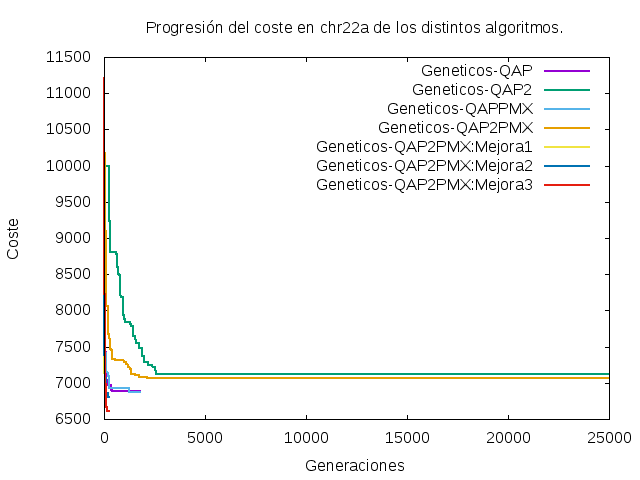
\includegraphics[width=0.7\linewidth]{graficos/comparativachr22a}
	\caption[Comparativa chr22a]{Comparativa chr22a}
	\label{fig:comparativachr22a}
\end{figure}

En este gráfico se ve claramente que se han obtenido muchas generaciones en los algoritmos genéticos estacionarios mientras que tanto los meméticos como los generacionales han utilizado menos generaciones. Sin embargo, ambos han conseguido rebajar mucho más rápido la función de coste, incluso han superado el mínimo local en el que se han quedado estancados los algoritmos estacionarios.\\

Esto no ocurre en otras instancias, como por ejemplo en $sko81$:\\

\begin{figure}[H]
	\centering
	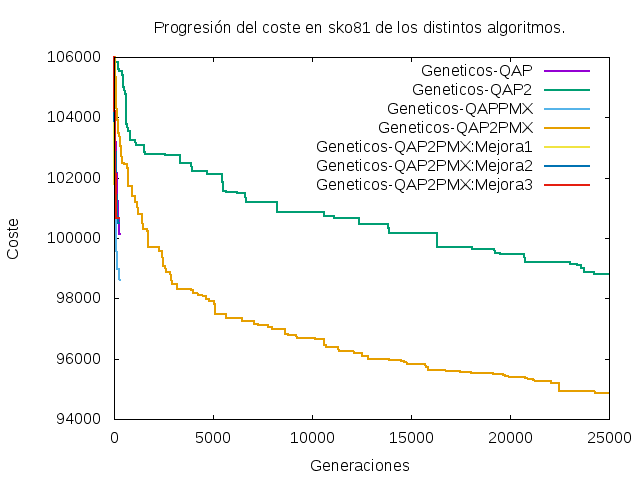
\includegraphics[width=0.7\linewidth]{graficos/comparativasko81}
	\caption[Comparativa sko81]{Comparativa sko81}
	\label{fig:comparativasko81}
\end{figure}

Este gráfico nos muestra que, con las iteraciones máximas que le hemos puesto, los algoritmos tanto meméticos como generacionales no han tenido tiempo de dar una solución de calidad. Sin embargo, los algoritmos estacionarios si han podido ir mejorando su coste de forma progresiva. En los siguientes dos casos se tienen comportamientos similares, solo que en la pocas iteraciones si que se ha conseguido un coste parecido:\\

\begin{figure}[H]
	\centering
	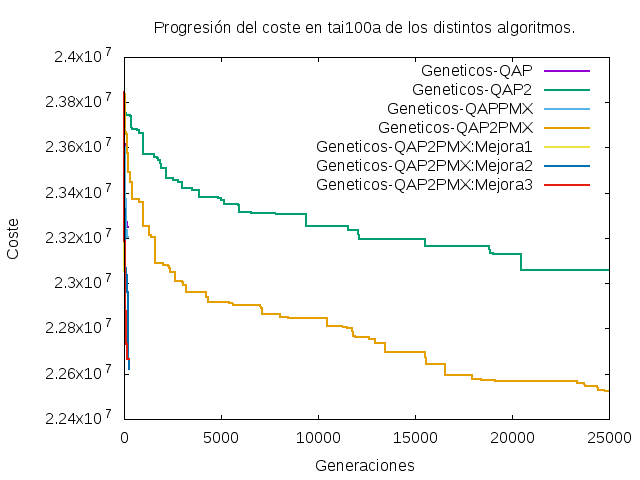
\includegraphics[width=0.7\linewidth]{graficos/comparativatai100a}
	\caption[Comparativa tai100a]{Comparativa tai100a}
	\label{fig:comparativatai100a}
\end{figure}

\begin{figure}[H]
	\centering
	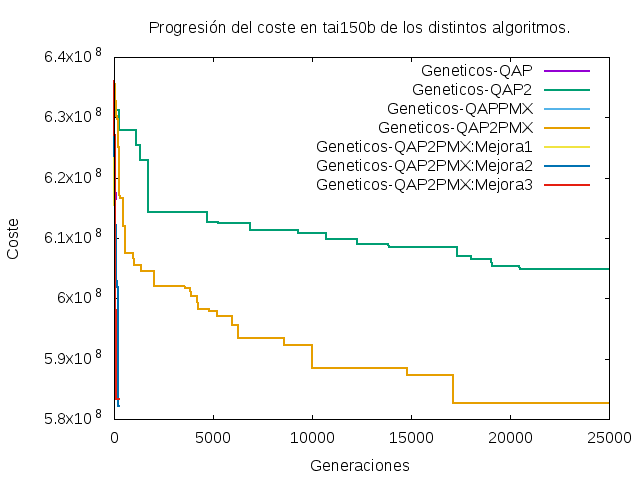
\includegraphics[width=0.7\linewidth]{graficos/comparativatai150b}
	\caption[Comparativa tai150b]{Comparativa tai150b}
	\label{fig:comparativatai150b}
\end{figure}

Por último, en la instancia más grande(tai256c) no se consigue apenas una mejora consistente, volvemos al caso de  sko81:\\

\begin{figure}[H]
\centering
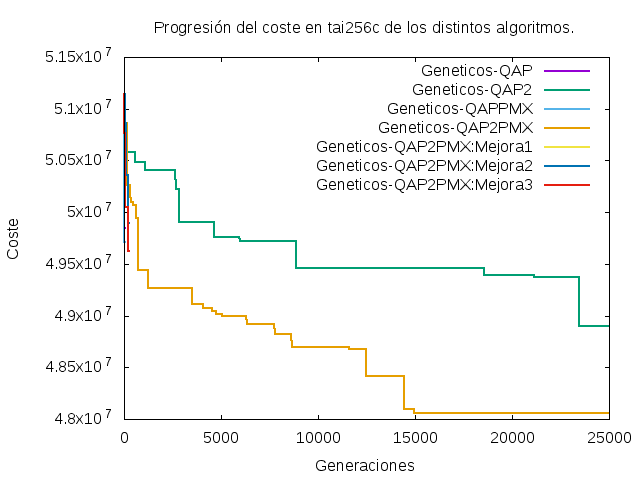
\includegraphics[width=0.7\linewidth]{graficos/comparativatai256c}
\caption[]{Comparativa 256c}
\label{fig:comparativatai256c}
\end{figure}

\subsection{Análisis de AG generacionales.}

En las gráficas antes vistas se puede observar fácilmente el comportamiento de los algoritmos estacionarios ya que tienen muchas generaciones. Veamos ahora el comportamiento en concreto de los algoritmos generacionales y meméticos:

\begin{figure}[H]
\centering
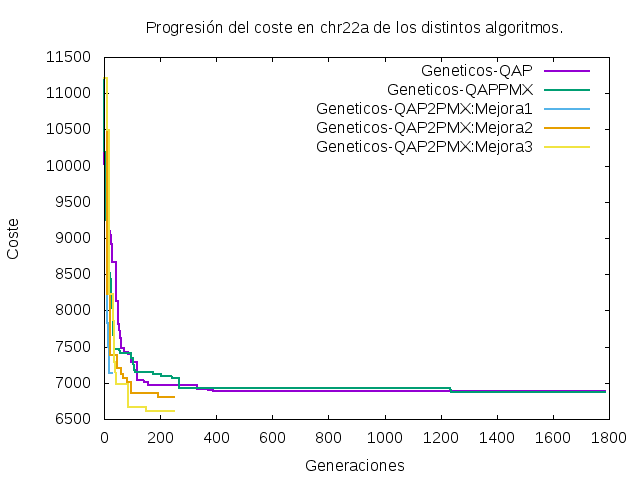
\includegraphics[width=0.7\linewidth]{graficos/comparativaGeneracionalchr22a}
\caption{Comparativa generacional vs meméticos estacionarios chr22a}
\label{fig:comparativaGeneracionalchr22a}
\end{figure}

Lo primero que notamos en esta comparativa es que, aun evaluando muchísimas veces la función objetivo en cada generación de los algoritmos genéticos generacionales, en un problema de tamaño pequeño los algoritmos meméticos utilizan muy pocas generaciones en comparación. Esto se debe a la cantidad de mutaciones que hacemos. Veamos que ocurre en las siguientes instancias:\\

\begin{figure}[H]
\centering
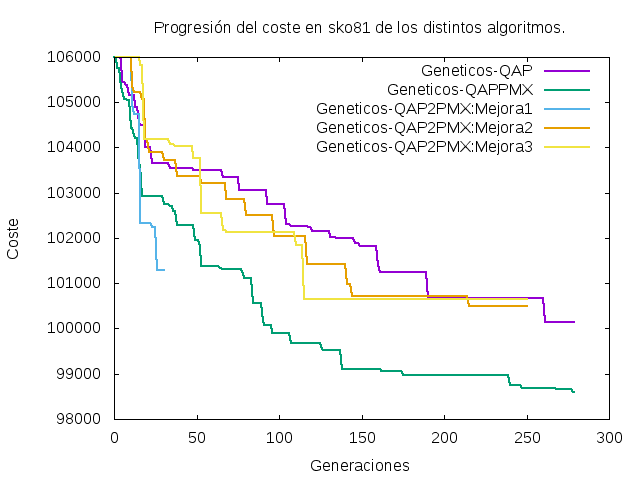
\includegraphics[width=0.7\linewidth]{graficos/comparativaGeneracionalsko81}
\caption{Comparativa generacional vs meméticos estacionarios sko81}
\label{fig:comparativaGeneracionalsko81}
\end{figure}

En esta instancia el número de generaciones se igualan ya que se evalúa más veces la función objetivo gracias a las mutaciones. También se puede observar que la evolución de los algoritmos meméticos se produce a saltos. Otro dato importante a tener en cuenta es que, pese a tener mejor estadístico la tercera mejora,  en esta instancia la segunda mejora lo supera. La primera mejora tiene muchas menos iteraciones ya que utiliza la mayoría de las evaluaciones de la función coste en búsquedas locales.\\

En los siguientes gráficos se ve cómo decrece el número de generaciones de los algoritmos genéticos generacionales mientras que los meméticos estacionarios mantienen sus generaciones fijas:\\

\begin{figure}[H]
	\centering
	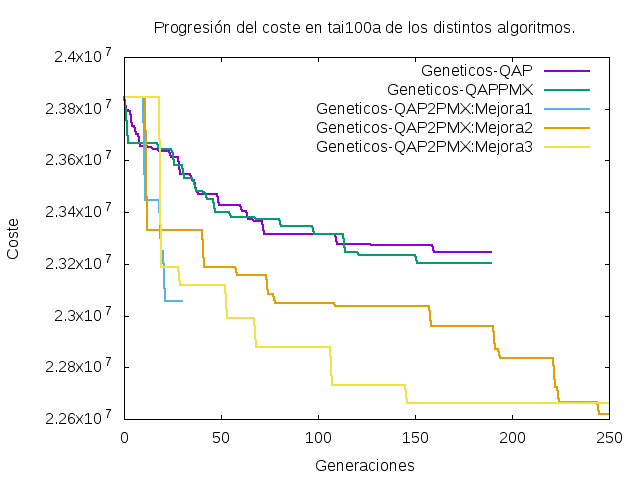
\includegraphics[width=0.7\linewidth]{graficos/comparativaGeneracionaltai100a}
	\caption{Comparativa generacional vs meméticos estacionarios tai100a}
	\label{fig:comparativaGeneracionaltai100a}
\end{figure}
 
\begin{figure}[H]
\centering
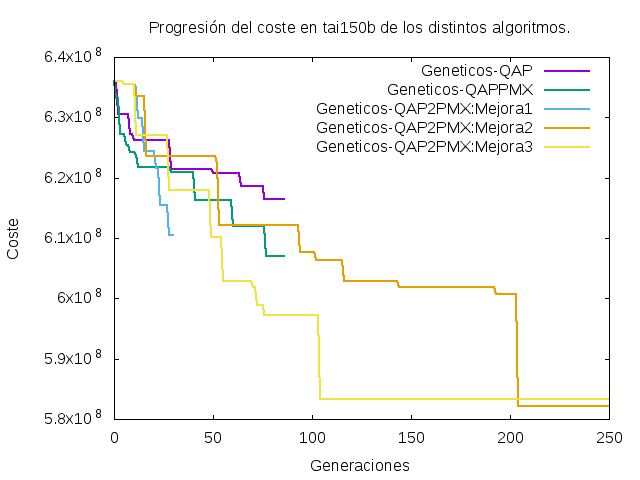
\includegraphics[width=0.7\linewidth]{graficos/comparativaGeneracionaltai150b}
\caption{Comparativa generacional vs meméticos estacionarios tai150b}
\label{fig:comparativaGeneracionaltai150b}
\end{figure}

\begin{figure}[H]
\centering
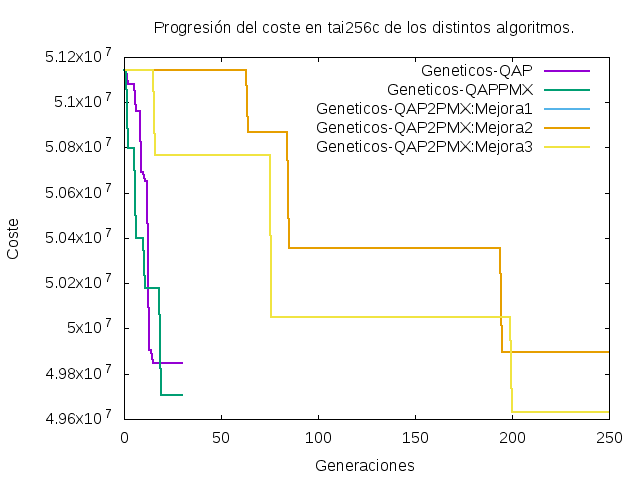
\includegraphics[width=0.7\linewidth]{graficos/comparativaGeneracionaltai256c}
\caption{Comparativa generacional vs meméticos estacionarios tai256c}
\label{fig:comparativaGeneracionaltai256c}
\end{figure}

\subsection{Posibles mejoras de los algoritmos}

Como ya se dijo en el apartado de consideraciones de parada, hay varias ideas en los algoritmos que se deben pulir:\\

\begin{itemize}
	\item \textbf{Tiempo de ejecución.} Las mutaciones, aunque sean evaluaciones de la función objetivo, tardan mucho menos en ser evaluadas. Se debería poder evaluar muchas veces tales mutaciones sin que ello repercutiese demasiado en el número de evaluaciones totales.
	
	\item \textbf{Evaluaciones por BL}. En los algoritmos meméticos la búsqueda local solo dispone de 400 evaluaciones. Si consideramos los primeros 400 genes, nunca se podrá mejorar los últimos. Para poder solventar esto, se podría empezar a profundizar en cada búsqueda local en un gen distinto o incluso aleatorizar la selección del gen a investigar. Otra forma de poder mejorar este aspecto es que el número de evaluaciones de la búsqueda local asegurase que intenta cambiar y mejorar al menos una vez cada gen. Es decir, que en vez de tener un número fijo de evaluaciones(400), este número dependa del número de genes(posibles trasposiciones $(i,j)$).
	
	\item \textbf{Parámetros modificables.} Dependiendo del tamaño del problema podríamos modificar cada cuanto se debe realizar una búsqueda local en los algoritmos meméticos, ya que estos consumen muchas evaluaciones y no dejan al algoritmo genético evolucionar para producir diversidad. De hecho, la última mejora se podría considerar que se comporta casi como una búsqueda local multiarranque en algunos casos(aplicando siempre la búsqueda local a los mejores).
	
\end{itemize}








\end{document}





